\selectlanguage{italian}

Lo studio delle molecole, ed in particolare delle molecole diatomiche, permette di illustrare due concetti fondamentali nello studio della fisica della materia: la separazione adiabatica del moto elettronico da quello nucleare ed il legame chimico.

\section{Separazione adiabatica}

L'Hamiltoniana per un sistema generico di $ M $ nuclei ed $ N $ elettroni è:
\begin{equation}
	\mathcal{H} = T_n + T_e + V_{ne} + V_{nn} + V_{ee}
	\label{eq:mol-ham-tot}
\end{equation}
Sebbene la funzione d'onda totale del sistema $ \Psi(r,R) $ dipenda dalle coordinate $ r $ di tutti gli elettroni ed $ R $ di tutti i nuclei, è possibile semplificare il problema. Infatti, essendo le masse dei nuclei e quelle degli elettroni diverse di circa tre ordini di grandezza, si può considerare che anche le time-scales dei moti dei nuclei siano tre ordini di grandezza maggiori rispetto a quelle dei moti degli elettroni: c'è dunque un disaccoppiamento dei due moti\footnotemark, in quanto si può assumere che il moto nucleare non induca alcuna transizione sugli stati elettronici (poiché le energie dei moti nucleari sono troppo piccole per colmare i gap energetici tra stati elettronici), da cui il nome di \textit{separazione adiabatica} (o di Born-Oppenheimer).

\footnotetext{In maniera approssimativa, si può dire che gli elettroni percepiscono i nuclei come fermi, mentre i nuclei risentono solo degli effetti medi del moto elettronico.}

\begin{definition}{Fattorizzazione adiabatica}{}
	La funzione d'onda totale del sistema si fattorizza come:
	\begin{equation}
		\Psi(r,R) = \Phi(R) \psi_e(r,R)
	\end{equation}
	dove $ \Phi(R) $ è la \textit{funzione d'onda nucleare} e $ \psi_e(r,R) $ è la \textit{funzione d'onda elettronica}, la quale è soluzione dell'equazione d'onda elettronica:
	\begin{equation}
		[T_e + V_{ne}(r,R) + V_{ee}(r)] \psi_e^{(a)}(r,R) = E_e^{(a)}(R) \psi_e^{(a)}(r,R)
		\label{eq:mol-el-eq}
	\end{equation}
	con $ (a) $ set di autovalori.
\end{definition}

La funzione d'onda $ \psi_e^{(a)}(r,R) $ descrive un autostato elettronico per una geometria fissata dei nuclei: la dipendenza da $ R $ di $ \psi_e^{(a)}(r,R) $ ed $ E_e^{(a)}(R) $ è puramente parametrica.

\begin{proposition}{Equazione d'onda nucleare}{}
	La funzione d'onda nucleare $ \Phi(R) $ è soluzione dell'equazione d'onda nucleare:
	\begin{equation}
		[T_n + V_\text{ad}^{(a)}(R)] \Phi(R) = E_\text{tot} \Phi(R)
		\label{eq:mol-nucl-eq}
	\end{equation}
	dove il \textit{potenziale adiabatico totale} è:
	\begin{equation}
		V_\text{ad}^{(a)}(R) \equiv E_e^{(a)}(R) + V_{nn}(R)
		\label{eq:ad-pot}
	\end{equation}

	\tcblower

	\begin{proof}
		Partendo dall'Eq. \ref{eq:mol-ham-tot}:
		\begin{equation*}
			[T_n + T_e + V_{nn} + V_{ne} + V_{ee}] \Phi(R) \psi_e(r,R) = E_\text{tot} \Phi(R) \psi_e(r,R)
		\end{equation*}
		e notando che, essendo $ T_e \sim \lap_r $, si ha $ T_e [\Phi(R) \psi_e(r,R)] = \Phi(R) T_e \psi_e(r,R) $:
		\begin{equation*}
			- \sum_\alpha \frac{\hbar^2}{2M_\alpha} \lap_{R_\alpha} [\Phi(R) \psi_e(r,R)] + \Phi(R) \underbrace{[T_e + V_{nn} + V_{ne}] \psi_e(r,R)}_{\text{equazione elettronica}} + \Phi(R) V_{nn} \psi_e(r,R) = E_\text{tot} \Psi(r,R)
		\end{equation*}
		Il primo termine diventa:
		\begin{equation*}
			\begin{split}
				- \sum_\alpha \frac{\hbar^2}{2m_\alpha} \lap_{R_\alpha} [\Phi(R) \psi_e(r,R)]
				= & - \sum_\alpha \frac{\hbar^2}{2M_\alpha} [\Phi(R) \lap_{R_\alpha} \psi_e(r,R) + 2 \nabla_{R_\alpha} \Phi(R) \cdot \nabla_{R_\alpha} \psi_e(r,R)] \\
				& - \psi_e(r,R) \sum_\alpha \frac{\hbar^2}{2M_\alpha} \lap_{R_\alpha} \Phi(R)
			\end{split}
		\end{equation*}
		I primi due termini (non-adiabatici) possono essere ignorati in approssimazione adiabatica, così da rimanere solo col terzo:
		\begin{equation*}
			\psi_e^{(a)}(r,R) [T_n + E_e^{(a)}(R) + V_{nn}(R)] \Phi(R) = E_\text{tot} \Phi(R) \psi_e^{(a)}(r,R)
		\end{equation*}
		Moltiplicando per $ [\psi_e^{(a)}(r,R)]^* $ da sinistra ed integrando su tutte le $ r $ si ottiene infine la tesi.
	\end{proof}
\end{proposition}

L'equazione elettronica presenta, nel caso $ N > 1 $, le stesse complicazioni della trattazione dei MEAs, ed è ugualmente risolvibile col metodo HF (con l'ulteriore complicazione che ora bisogna considerare varie geometrie molecolari date dalle $ R $): una volta selezionato lo stato elettronico $ a $, esso segue adiabaticamente il moto nucleare, non transizionando ad altri stati $ a' \neq a $ (questa è un'approssimazione della realtà). \\
Per quanto riguarda l'equazione nucleare, essa esprime il moto dei nuclei all'interno del potenziale adiabatico totale, composto da un termine Coulombiano repulsivo ed un contributo elettronico attrattivo (è ciò che permette alle molecole di esistere come stati legati). $ V_\text{ad}^{(a)}(R) $, funzione di $ 3M $ variabili, presenta una simmetria roto-traslazionale: ciò suggerisce che esso dipenda dalle distanze relative tra i nuclei atomici. Un esempio di andamento di $ V_\text{ad}^{(a)}(R) $ è riportato in Fig. \ref{ad-pot} (per il ground state di una molecola diatomica): si vede che il potenziale ha un minimo $ R_\text{m} $ finito, attorno al quale avvengono le oscillazioni del moto nucleare a bassa temperatura.

\begin{figure}
	\centering
	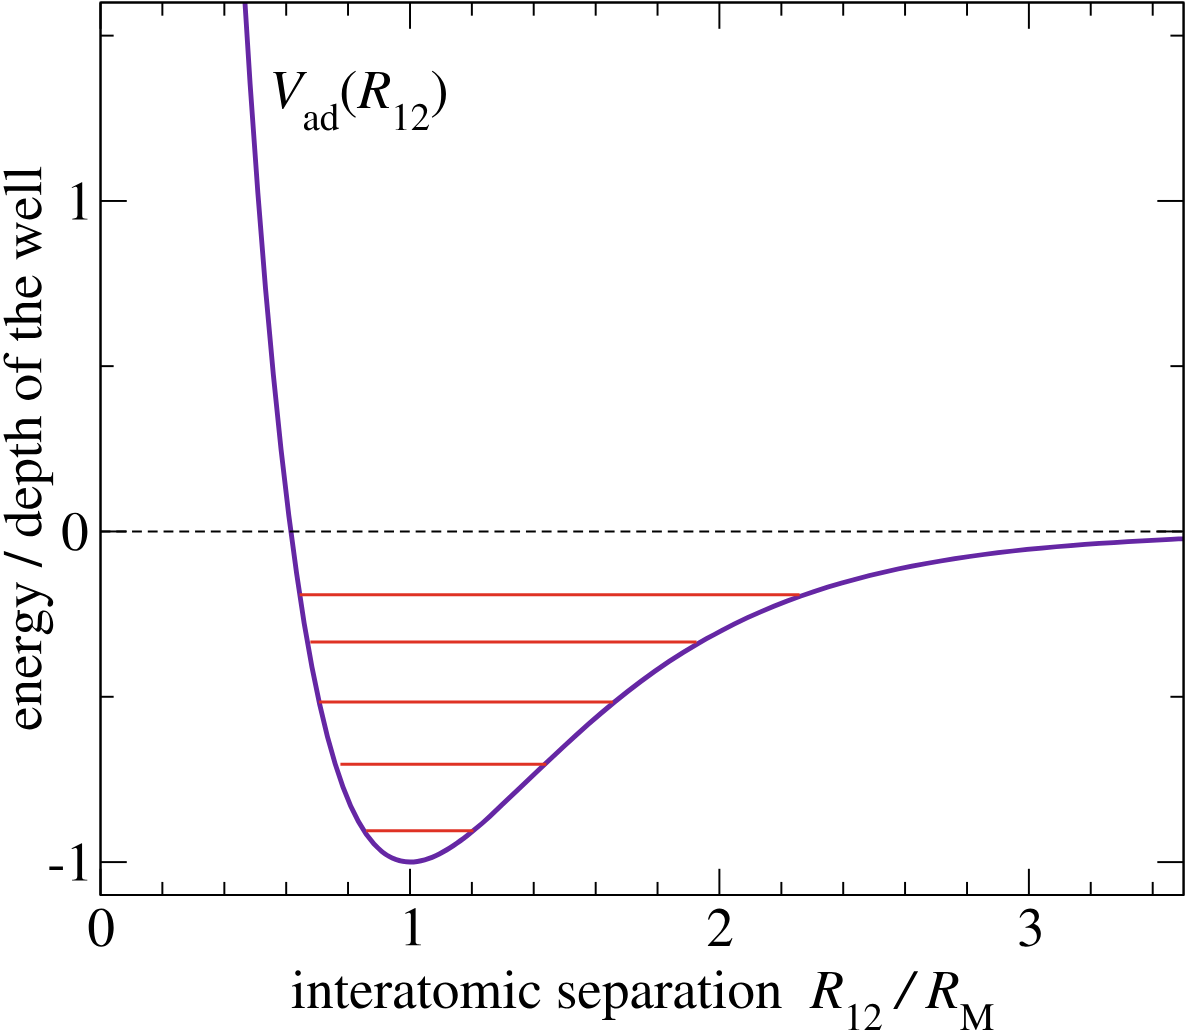
\includegraphics[width = 0.40 \textwidth]{adiabatic-potential.png}
	\caption{Adiabatic potential for a diatomic molecule.}
	\label{ad-pot}
\end{figure}

\section{Legami}

L'andamento del potenziale adiabatico in Fig. \ref{ad-pot} è alquanto generale, anche per molecole con $ M > 2 $, e pone le basi per lo studio di strutture molecolari complesse.

\subsection{\texorpdfstring{$ \ch{H_2^+} $}{H2+}}

Si consideri ad esempio la più semplice molecola diatomica: $ \ch{H_2^+} $. In questo caso non è presente alcuna repulsione elettrone-elettrone, dunque sull'unico elettrone agisce esclusivamente $ V_{ne} = V_\text{L} + V_\text{R} $, dove $ \text{L},\text{R} $ si riferiscono rispettivamente al nucleo sinistro o destro (arbitrariamente scelto il verso dell'asse molecolare $ \hat{\ve{e}}_z $): questi possono essere assunti fissi e posti a $ \pm R_{12}/2 $ lungo $ \hat{\ve{e}}_z $, dove $ \ve{R}_{12} \equiv \abs{\ve{R}_\text{L} - \ve{R}_\text{R}} $.

\begin{figure}[!b]
	\centering
	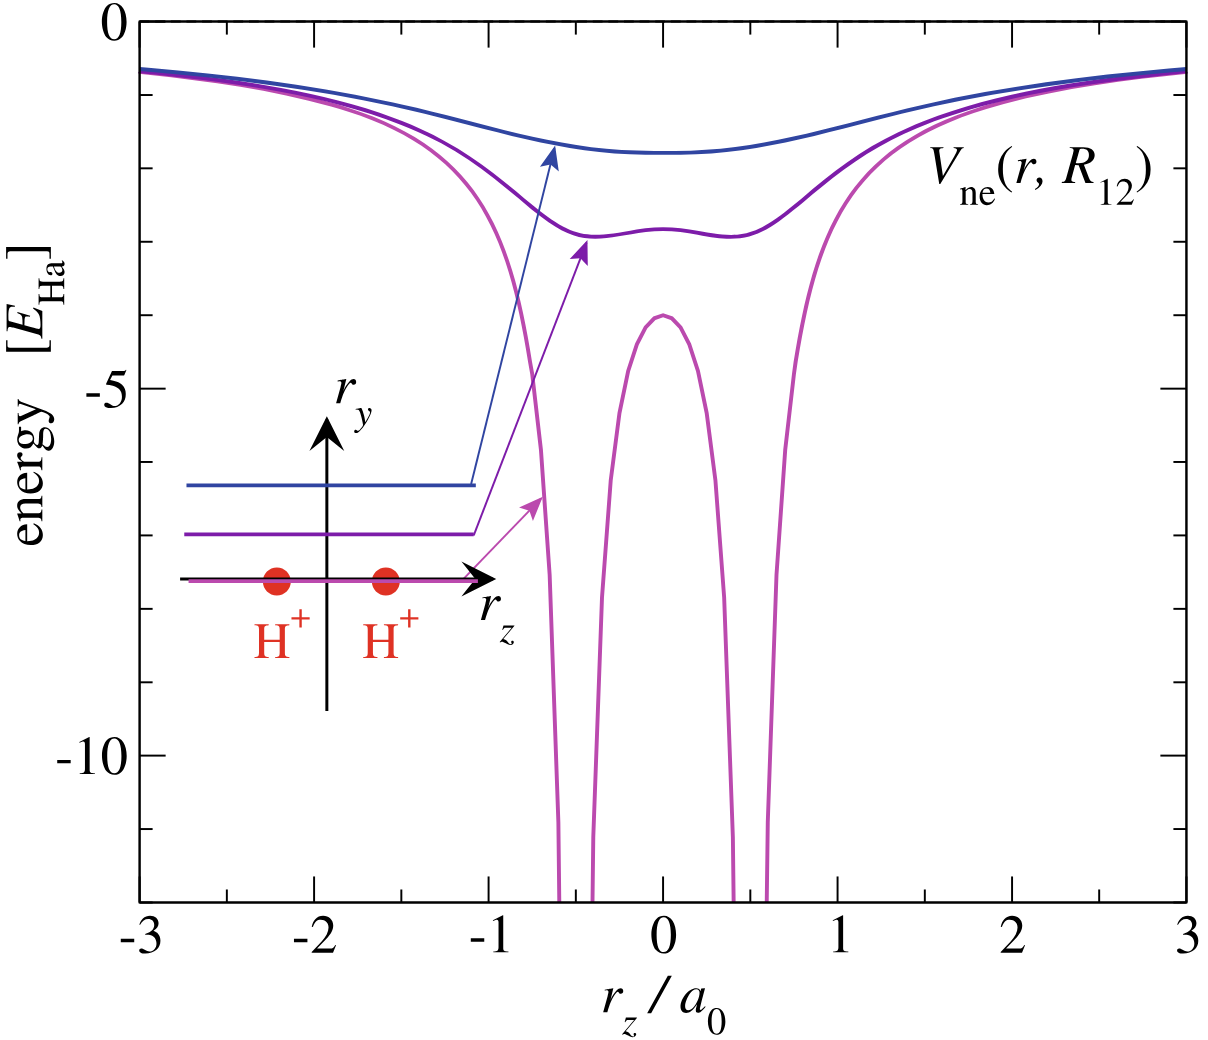
\includegraphics[width = 0.40 \textwidth]{ne-potential-h2.png}
	\caption{$ V_{ne} $ potential for the $ \ch{H_2^^+} $ molecule.}
	\label{ne-h2}
\end{figure}

Con riferimento alla Fig. \ref{ne-h2}, si noti che per $ -R_{12}/2 < r_z < R_{12}/2 $ il potenziale $ V_{ne}(r,R_{12}) $ è circa doppiamente negativo rispetto al caso atomico, suggerendo che l'elettrone potrebbe abbassare la propria energia potenziale media avendo una distribuzione di probabilità piccata nel mezzo dei due nuclei. Per verificare se ciò permette la formazione di un legame, bisogna confrontare che $ V_\text{ad}(R_{12}) < V_\text{ad}(\infty) = E_\text{1s} = -\frac{1}{2} E_\text{Ha} $ (poiché in tale limite si hanno praticamente un protone ed un atomo di idrogeno infinitamente separati, e $ \mu/m_e \approx 1 $). A tal fine, si adotta un approccio variazionale per verificare il valore dell'energia tramite la LCAO (Linear Combination of Atomic Orbitals): si considerino i due ground state atomici $ \ket{\text{1s};\text{L}} \equiv \ket{\text{L}} $ e $ \ket{\text{1s};\text{R}} \equiv \ket{\text{R}} $, assumendo $ \braket{\text{L} | \text{R}} > 0 $, e, data la simmetria assiale (cilindrica attorno $ \hat{\ve{e}}_z $) del problema, si considerino le combinazioni lineari opportunamente normalizzate (plottate in Fig. \ref{gs-h2}):
\begin{equation}
	\ket{\text{S}} = [2(1 + \braket{\text{L} | \text{R}})]^{-1/2} (\ket{\text{L}} + \ket{\text{R}})
	\qquad \qquad
	\ket{\text{A}} = [2(1 - \braket{\text{L} | \text{R}})]^{-1/2} (\ket{\text{L}} - \ket{\text{R}})
	\label{eq:h2-kets}
\end{equation}

\begin{figure}[!b]
	\centering
	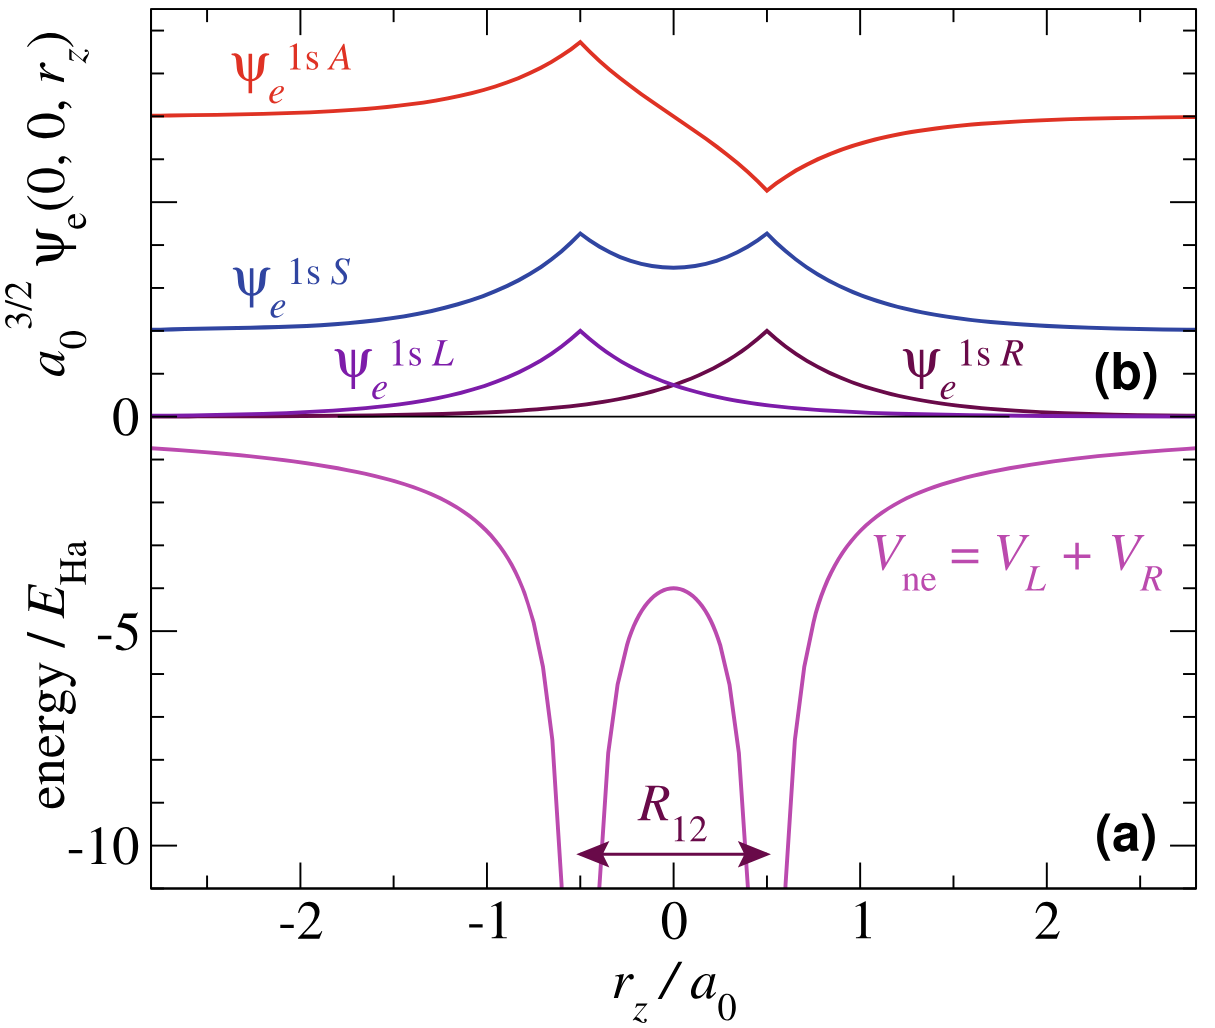
\includegraphics[width = 0.50 \textwidth]{symm-asymm-h2.png}
	\caption{Symmetric and antisymmetric LCAO for the ground state of $ \ch{H_2^+} $.}
	\label{gs-h2}
\end{figure}

Per il principio variazionale, per l'energia del ground state vale $ E_e^{(\text{gs})}(R_{12}) \le \braket{\text{S}/\text{A} | T_e + V_{ne} | \text{S}/\text{A}} \equiv \mathcal{E}_{\text{S},\text{A}} \,\,\forall R_{12} \in \R_+ $.

\begin{proposition}{}{}
	A grande distanza $ R_{12} \gg a_0 $ si ha:
	\begin{equation}
		\mathcal{E}_{\text{S},\text{A}} + \frac{E_\text{Ha}}{2} \simeq - \frac{e^2}{R_{12}} (1 \pm \braket{\text{L} | \text{R}})
		\label{eq:h2-symm-asymm}
	\end{equation}

	\tcblower

	\begin{proof}
		Per calcolo diretto:
		\begin{equation*}
			\begin{split}
				\mathcal{E}_\text{\text{S},\text{A}}
				& = \braket{\text{S}/\text{A} | T_e + V_{ne} | \text{S}/\text{A}} = \frac{\braket{\text{L} | T_e + V_{ne} | \text{L}} \pm \braket{\text{R} | T_e + V_{ne} | \text{L}} + (\text{L} \leftrightarrow \text{R})}{2 (1 \pm \braket{\text{L} | \text{R}})} \\
				& = \frac{\braket{\text{L} | T_e + V_\text{L} | \text{L}} + \braket{\text{L} | V_\text{R} | \text{L}} \pm \braket{\text{R} | T_e + V_\text{L} | \text{L}} \pm \braket{\text{R} | V_\text{R} | \text{L}}}{1 \pm \braket{\text{L} | \text{R}}} = - \frac{E_\text{Ha}}{2} + \frac{\braket{\text{L} | V_\text{R} | \text{L}} \pm \braket{\text{R} | V_\text{R} | \text{L}}}{1 \pm \braket{\text{L} | \text{R}}}
			\end{split}
		\end{equation*}
		essendo $ \ket{\text{L}} $ autostato di $ T_e + V_\text{L} $ con autovalore $ -E_\text{Ha}/2 $. I due elementi di matrice di $ V_\text{R} $ sono entrambi funzioni reali e negative di $ R_{12} $: il termine $ \braket{\text{L} | V_\text{R} | \text{L}} $ rappresenta l'attrazione che il nucleo destro esercita sull'elettrone orbitante attorno al nucleo sinistro, dunque per $ R_{12} $ abbastanza grande si ha:
		\begin{equation*}
			\braket{\text{L} | V_\text{R} | \text{L}} \simeq - \frac{e^2}{R_{12}}
		\end{equation*}
		Il termine $ \braket{\text{R} | V_\text{R} | \text{L}} $, d'altro canto, può essere approssimato considerando che la distribuzione $ \psi_\text{L}(\ve{r}) \psi_\text{R}(\ve{r}) $ è piccata nella regione assiale tra i due nuclei, al centro della quale $ V_\text{R} \simeq - \frac{e^2}{R_{12}/2} $, così che:
		\begin{equation*}
			\braket{\text{R} | V_\text{R} | V_\text{L}} \simeq - \frac{e^2}{R_{12}} 2\braket{\text{L} | \text{R}}
		\end{equation*}
		Si può quindi espandere l'espressione totale considerando $ \braket{\text{L} | \text{R}} $ sufficientemente piccolo:
		\begin{equation*}
			\mathcal{E}_{\text{S},\text{A}} + \frac{E_\text{Ha}}{2} \simeq - \frac{e^2}{R_{12}} \frac{1 \pm 2 \braket{\text{L} | \text{R}}}{1 \pm \braket{\text{L} | \text{R}}} \simeq - \frac{e^2}{R_{12}} (1 \pm \braket{\text{L} | \text{R}})(1 \mp \braket{\text{L} | \text{R}}) \simeq - \frac{e^2}{R_{12}} (1 \pm \braket{\text{L} | \text{R}})
		\end{equation*}
		che è il risultato cercato.
	\end{proof}
\end{proposition}

L'Eq. \ref{eq:h2-symm-asymm} mostra come $ \mathcal{E} + \frac{E_\text{Ha}}{2} + V_{nn} $, con $ V_{nn} = \frac{e^2}{R_{12}} $, sia negativo per $ \ket{\text{S}} $ e positivo per $ \ket{\text{A}} $: ciò significa che la repulsione tra i due nuclei è vinta solo dalla LCAO simmetrica, nel qual caso di forma effettivamente un \textit{legame}. \\
Si può anche considerare il risultato esatto per $ R_{12} $ generico (plottato in Fig. \ref{h2-en}):
\begin{equation}
	\mathcal{E}_{\text{S},\text{A}} = - \frac{E_\text{Ha}}{2} + \frac{\braket{\text{L} | V_\text{R} | \text{L}} \pm \braket{\text{R} | V_\text{R} | \text{L}}}{1 \pm \braket{\text{L} | \text{R}}}
\end{equation}

\begin{figure}[!b]
	\centering
	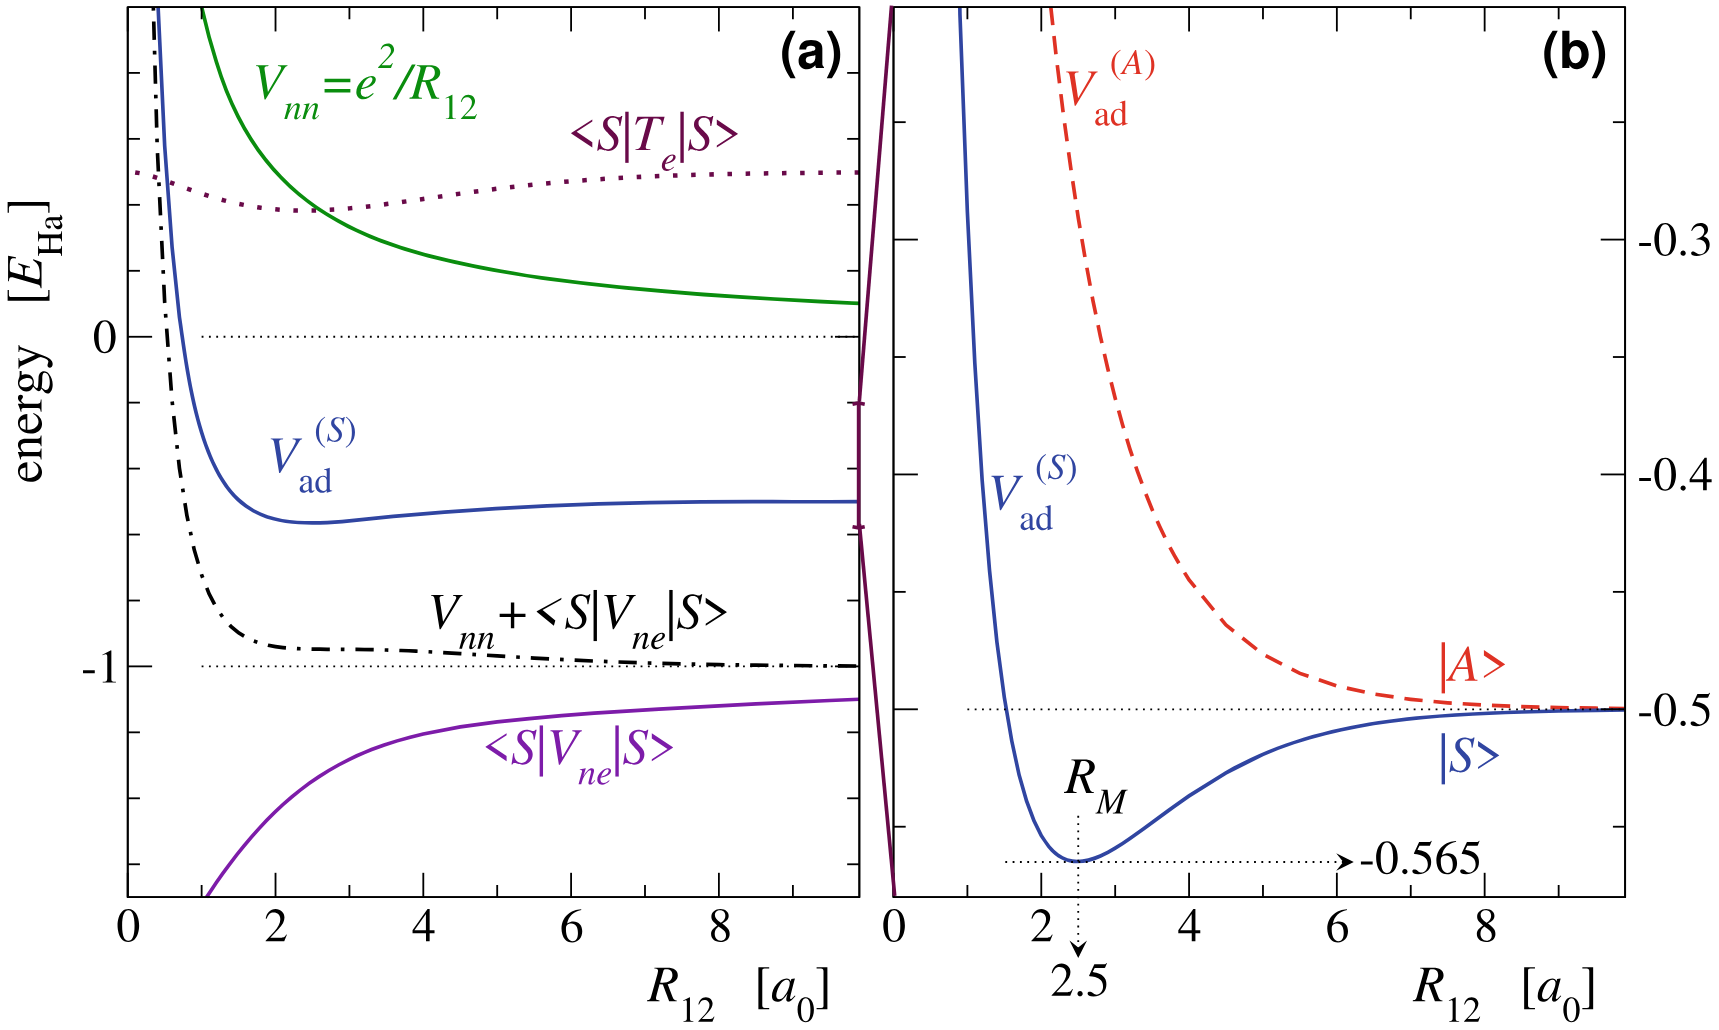
\includegraphics[width = 0.70 \textwidth]{h2-en.png}
	\caption{Total adiabatic potential for $ \ket{\text{S}} $ and $ \ket{\text{A}} $.}
	\label{h2-en}
\end{figure}

Si possono fare alcune osservazioni:
\begin{enumerate}
	\item $ V_\text{ad}^{(\text{S})}(R_{12}) $ presenta un minimo per $ R_{12} = R_\text{m} \simeq 2.5 a_0 $, e questa buca di potenziale è abbastanza profonda da legare i due protoni, pertanto $ \ket{\text{S}} $ è detto \textit{stato legante};
	\item $ V_\text{ad}^{(\text{A})}(R_{12}) $ è monotonamente decrescente, ovvero è un potenziale puramente repulsivo, dunque $ \ket{\text{A}} $ è detto \textit{stato anti-legante};
	\item per $ R_{12} < R_\text{m} $ entrambi i potenziali adiabatici divergono a causa di una singolarità in $ V_{nn} $, il quale non è più efficacemente schermato, ed anche perché gli elettroni sono costretti a muoversi in una buca di potenziale più stretta, dunque con un'energia cinetica maggiore (per il principio d'indeterminazione).
\end{enumerate}
In definitiva, il legame in $ \ch{H_2^+} $ è dovuto sia ad un abbassamento dell'energia cinetica elettronica (poiché l'elettrone si muove in una buca di potenziale più larga) e ad un abbassamento dell'energia potenziale del sistema (poiché l'elettrone scherma la repulsione tra i due nuclei tramite una distribuzione di probabilità piccata nel mezzo). \\
Questo modello variazionale è valido per $ \braket{\text{L} | \text{R}} \ll 1 $, ovvero $ R_{12} \gg a_0 $, ma diventa particolarmente inaccurato per $ R_{12} $ piccolo, poiché in tal caso nella LCAO vanno considerati anche gli stati diversi da $ \text{1s} $: il modello variazionale dà energia di legame molecolare $ V_\text{ad}^{(\text{S})}(\infty) - V_\text{ad}^{(\text{S})}(R_\text{m}) \simeq 1.76\ev $ con $ R_\text{m} = 2.50 a_0 $, mentre il valore sperimentale è $ 2.79\ev $ con $ R_\text{m} = 2.00 a_0 $.

\paragraph{Numeri quantici}

La simmetria di $ \ch{H_2^+} $ è cilindrica, dunque soltanto $ L_z $ può essere diagonalizzato\footnote{In coordinate cilindriche $ \ve{r} = (\rho \cos \varphi, \rho \sin \varphi, z) $ e $ \hat{L}_z \defeq -i\hbar (x \pa_y - y \pa_x) = -i \hbar \pa_\varphi $, quindi le sue autofunzioni sono $ f(\varphi) = \mathcal{N} e^{i m \varphi} $. La condizione di periodicità $ f(\varphi) = f(\varphi + 2\pi) $ impone $ m \in \Z $.}: l'unico numerico quantico $ \virgolette{buono} $ è $ m $. In base al valore di $ \abs{m} = 0, 1, 2, \dots $ si indicano gli stati con $ \sigma, \pi, \delta, \dots $; inoltre, gli stati anti-leganti acquistano un asterisco. Si noti che, a parte gli stati $ \sigma $, tutti questi stati sono doppiamente degeneri ($ \pm m $). Questa degenerazione è dovuta a una simmetria dell'Hamiltoniana. In particolare, in assenza di campi magnetici esterni, essa è simmetrica per $ \sigma_\text{v} : \varphi \mapsto -\varphi $, ovvero una riflessione rispetto al piano che contiene l'asse molecolare, la quale implica che l'energia sia $ E = E(\abs{m}) $. Nel caso di molecole diatomiche omonucleari, inoltre, si hanno due ulteriori simmetrie. La prima è la simmetria sotto riflessione rispetto al piano ortogonale all'asse molecolare, denominata $\sigma_\text{n}: z \mapsto -z$, e la seconda è una rotazione di $\pi$: $x \mapsto -x, y \mapsto -y$. La combinazione delle due costituisce l'inversione $ \sigma_\text{i} : \ve{r} \mapsto -\ve{r}$: in base all'autovalore di $ \sigma_\text{i} $, si distingue tra stati $ g $ (gerade, con $ +1 $) e $ u $ (ungerade, con $ -1 $).

\begin{example}{Stati $ \ket{\text{S}},\ket{\text{A}} $ in $ \ch{H_2^+} $}{}
	Gli stati $ \ket{\text{S}},\ket{\text{A}} $, definiti in Eq. \ref{eq:h2-kets}, sono LCAO di soli stati $ \text{1s} $, dunque sono stati $ \sigma $: in particolare, $ \ket{\text{S}} \equiv 1\sigma $ e $ \ket{\text{A}} \equiv 1\sigma^* $.
\end{example}



\subsubsection{Derivazione alternativa}

Si consideri la generica combinazione lineare $ \psi_e(r_1,r_2,R) = c_1 \psi_\text{1s}^{(1)}(r_1) + c_2 \psi_\text{1s}^{(2)}(r_2) $, con $ \ve{r}_{1,2} \equiv \ve{r} - \ve{R}_{1,2} $ e dipendenza parametrica da $ \ve{R} \equiv \ve{R}_1 - \ve{R}_2 $ (ricordare che $ \psi_\text{1s}(r) = \frac{1}{\sqrt{4\pi}} \frac{2}{a_0^{2/3}} \exp -r/a_0 $). Il metodo variazionale impone:
\begin{equation}
	\delta( \braket{\psi_e | \mathcal{H} | \psi_e} - E \braket{\psi_e | \psi_e}) = 0
	\label{eq:h2-var}
\end{equation}
Innanzitutto, si calcola:
\begin{equation*}
	\begin{split}
		\braket{\psi_e | \psi_e}
		& = \abs{c_1}^2 + \abs{c_2}^2 + c_1^* c_2 \int d^3r\, \psi_\text{1s}^{(1)*}(r_1) \psi_\text{1s}^{(2)}(r_2) + c_1 c_2^* \int d^3r\, \psi_\text{1s}^{(1)}(r_1) \psi_\text{1s}^{(2)*}(r_2) \\
		& \equiv \abs{c_1}^2 + \abs{c_2}^2 + c_1^* c_2 S_{12}(R) + c_1 c_2^* S_{12}^*(R)
	\end{split}
\end{equation*}
Inoltre, si trova:
\begin{equation*}
	\braket{\psi_e | \mathcal{H} | \psi_e} = \abs{c_1}^2 H_{11} + \abs{c_2}^2 H_{22} + c_1^* c_2 H_{12} + c_1 c_2^* H_{12}^*
\end{equation*}
con:
\begin{equation*}
	\begin{split}
		H_{11} = \int d^3r\, \psi_\text{1s}^{(1)*}(r_1) \left[ - \frac{\hbar^2 \lap}{2m_e} - \frac{e^2}{r_1} - \frac{e^2}{r_2} \right] \psi_\text{1s}^{(1)}(r_1)
		& = - \frac{E_\text{Ha}}{2} + \int d^3\, \psi_\text{1s}^{(1)*}(r_1) \left( -\frac{e^2}{r_2} \right) \psi_\text{1s}^{(1)}(r_1) \\
		& \equiv - \frac{E_\text{Ha}}{2} + J_1(R)
	\end{split}
\end{equation*}
\begin{equation*}
	\begin{split}
		H_{12} = \int d^3r\, \psi_\text{1s}^{(1)*}(r_1) \left[ - \frac{\hbar^2 \lap}{2m_e} - \frac{e^2}{r_1} - \frac{e^2}{r_2} \right] \psi_\text{1s}^{(2)}(r_2)
		& = - \frac{E_\text{Ha}}{2} S_{12}(R) + \int d^3r\, \psi_\text{1s}^{(1)*}(r_1) \left( - \frac{e^2}{r_1} \right) \psi_\text{1s}^{(2)}(r_2) \\
		\equiv - \frac{E_\text{Ha}}{2} S_{12}(R) + K_{12}(R)
	\end{split}
\end{equation*}
Per molecole omonucleari si trova $ H_{22} = H_{11} $, mentre in generale essi saranno diversi.
La variazione in Eq. \ref{eq:h2-var} avviene rispetto a $ c_1 $ e $ c_2 $, dunque imponendo le derivate parziali rispetto ad entrambi nulle si trova:
\begin{equation*}
	\begin{cases}
		c_1^* H_{11} + c_2^* H_{12}^* - E (c_1^* + c_2^* S_{12}^*) = 0 \\
		c_2^* H_{22} + c_1^* H_{12} - E (c_2^* - c_1^* S_{12}) = 0
	\end{cases}
	\qquad \iff \qquad
	\begin{vmatrix}
		H_{11} - E & H_{12}^* - E S_{12}^* \\
		H_{12} - E S_{12} & H_{22} - E
	\end{vmatrix}
	= 0
\end{equation*}
Questa matrice ha due autovalori (e due autovettori), che nel caso omonucleare sono:
\begin{equation*}
	E_\pm = \frac{H_{12} \mp H_{12}}{1 \mp S_{12}}
	\qquad \qquad
	\begin{pmatrix}
		c_1 \\ c_2
	\end{pmatrix}
	=
	\begin{pmatrix}
		1 \\ \pm 1
	\end{pmatrix}
\end{equation*}
In maniera esplicita:
\begin{equation}
	E_\pm(R) = - \frac{E_\text{Ha}}{2} + \frac{J_{1}(R) \mp K_{12}(R)}{1 \mp S_{12}(R)}
\end{equation}
che equivale all'Eq. \ref{eq:h2-symm-asymm}. Si vede che il legame non è dovuto all'integrale Coulombiano $ J_1(R) $, bensì all'integrale di risonanza $ K_{12}(R) $, il quale non ha un'interpretazione classica. Ovviamente tale modello è solo approssimato, ed una maggiore sovrapposizione coi dati sperimentali si potrebbe ottenere considerando altri stati oltre $ \text{1s} $ nella LCAO.

\subsection{Legami covalenti e ionici}

\subsubsection{Dimeri}

Il legame in $ \ch{H_2^+} $ non è un vero e proprio legame chimico, in quanto non c'è una coppia di elettroni che occupa lo stesso orbitale legante (legame covalente): questo è invece il caso di $ \ch{H_2} $, le cui autofunzioni per gli orbitali vanno determinate con metodi che considerino la repulsione elettrone-elettrone (come il metodo HF). Ad ogni modo, si trova un potenziale simile al potenziale adiabatico in Fig. \ref{ad-pot}; un tale potenziale ammette anche elettroni in stati eccitati: se entrambi si trovano nello stesso orbitale legante, allora la molecola esiste in uno stato legato, sebbene con binding energy minore rispetto a $ 1\sigma $. \\
Considerando atomi con $ Z $ via via maggiore, si vengono a formare molecole diatomiche omonucleari (o \textit{dimeri}) con un maggior numero di orbitali leganti/anti-leganti. Si evidenziano alcune proprietà:
\begin{enumerate}
	\item gli orbitali leganti sono sempre energeticamente inferiori rispetto ai corrispettivi anti-leganti;
	\item la forza di un legame covalente aumenta all'aumentare dell'ordine di legame, ovvero del numero di coppie di elettroni (di spin opposto, per il principio d'esclusione\footnotemark) presenti nell'orbitale legante ed assenti nel corrispettivo orbitale anti-legante (il più forte è $ \ch{N_2} $, con $ 10\ev $);
	\item nel riempimento della shell $ \text{2p} $, si ha un inversione per la quale gli orbitali $ 2\pi $ sono energeticamente inferiori a quelli $ 2\sigma $ (nonostante ci sia più overlap tra gli orbitali $ 2p_z $ (lungo l'asse molecolare) che formano $ 2\sigma $ rispetto agli orbitali $ 2p_x , 2p_y $ che formano $ 2\pi $); l'ordinamento $ \virgolette{normale} $ viene ristabilito da $ \ch{O_2} $ in poi.
\end{enumerate}

\footnotetext{Si noti che, considerando lo spin, gli orbitali $ \sigma $ possono contenere 2 elettroni, tutti gli altri orbitali 4 (poiché già doppiamente degeneri per $ \pm m $).}

\begin{figure}
	\centering
	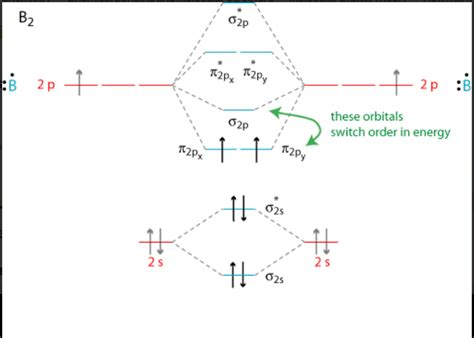
\includegraphics[width = 0.50 \textwidth]{sigma-pi-b2.jpg}
	\caption{Bonding orbitals (only for valence electrons) for $ \ch{B_2} $.}
	\label{bond-b2}
\end{figure}

Prendendo il caso di $ \ch{B_2} $ (o anche $ \ch{O_2} $), gli ultimi due elettroni di valenza vanno disposti per l'Aufbau su un orbitale $ \pi $ (o $ \pi^* $), il quale può però ospitare quattro elettroni: di conseguenza, per la prima regola di Hund essi occupano l'orbitale con spin paralleli. \\
Vengono osservati anche dimeri come $ \ch{Be_2} $ e $ \ch{Ne_2} $ che, nonostante un ordine di legame nullo, manifestano un debole legame non chimico (legame di van der Waals).

\paragraph{Potenziali analitici}

È possibile formulare alcuni modelli analitici per approssimare il potenziale adiabatico. Un esempio è il \textit{potenziale di Lennard-Jones}:
\begin{equation}
	V_\text{LJ}(R) = 4 \varepsilon \left[ \left( \frac{\sigma}{R} \right)^{12} - \left( \frac{\sigma}{R} \right)^6 \right]
\end{equation}
con $ \varepsilon \sim 1-100 \,\text{meV} $ e $ \sigma \sim 1-3 \ang $. Questo potenziale descrive i dimeri di atomi i cui orbitali sono completamente pieni (ovvero i gas nobili): essi infatti non formano legami covalenti, ma legami dovuti a deboli fluttuazioni indotte sui dipoli elettrici\footnotemark (che altrimenti sarebbero nulli). Ponendo $ V_\text{LJ}' = 0 $ si trova la distanza d'equilibrio $ R_\text{m} = \sqrt[6]{2} \sigma $ e la profondità della buca di potenziale $ V_\text{LJ}(R_\text{m}) = -\varepsilon $ (si noti che questi valori valgono per soli dimeri, in quanto molecole poliatomiche hanno geometrie più complesse). \\
Per descrivere legami covalenti si utilizza invece il \textit{potenziale di Morse}:
\begin{equation}
	V_\text{M}(R) = \mathcal{E}_d \left[ 1 - e^{-\beta (R - R_\text{m})} \right]^2
\end{equation}
dove $ \mathcal{E}_d $ è l'energia di dissociazione della molecola e $ \beta $ è un parametro legato alla frequenza caratteristica delle oscillazioni attorno al minimo di potenziale da $ \kappa = 2 \mathcal{E}_d \beta^2 $. A differenza di $ V_\text{LJ}(R) $, il potenziale di Morse ha un valore finito per $ R = 0 $.

\footnotetext{Un dipolo istantaneo $ \bs{\mu}_1 $ in un atomo induce un dipolo istantaneo indotto $ \bs{\mu}_2 $ sull'atomo adiacente: questo dipolo indotto avrà sempre verso opposto al primo dipolo, risultando dunque in un'interazione attrattiva tra di essi che scala come $ R^{-6} $.}

\subsubsection{Molecole diatomiche eteronucleari}

Sebbene i dimeri godano di una particolare simmetria per riflessioni, esistono anche molecole diatomiche eteronucleari. In questi casi, c'è un'asimmetria nella distribuzione di carica, poiché gli elettroni saranno maggiormente attratti da uno dei due atomi: come si vede in Fig. \ref{etero}, gli orbitali leganti si trovano energeticamente più vicini agli orbitali dell'atomo che li ha energeticamente più bassi, fino a casi limite come $ \ch{HF} $ in cui gli orbitali coincidono energeticamente. Si distingue quindi tra legami covalenti polari e legami ionici: di quest'ultimi si può dare una descrizione approssimata come di un completo trasferimento di carica dall'atomo meno elettronegativo a quello più elettronegativo (come in $ \ch{HF} $).

\begin{figure}
	\centering
	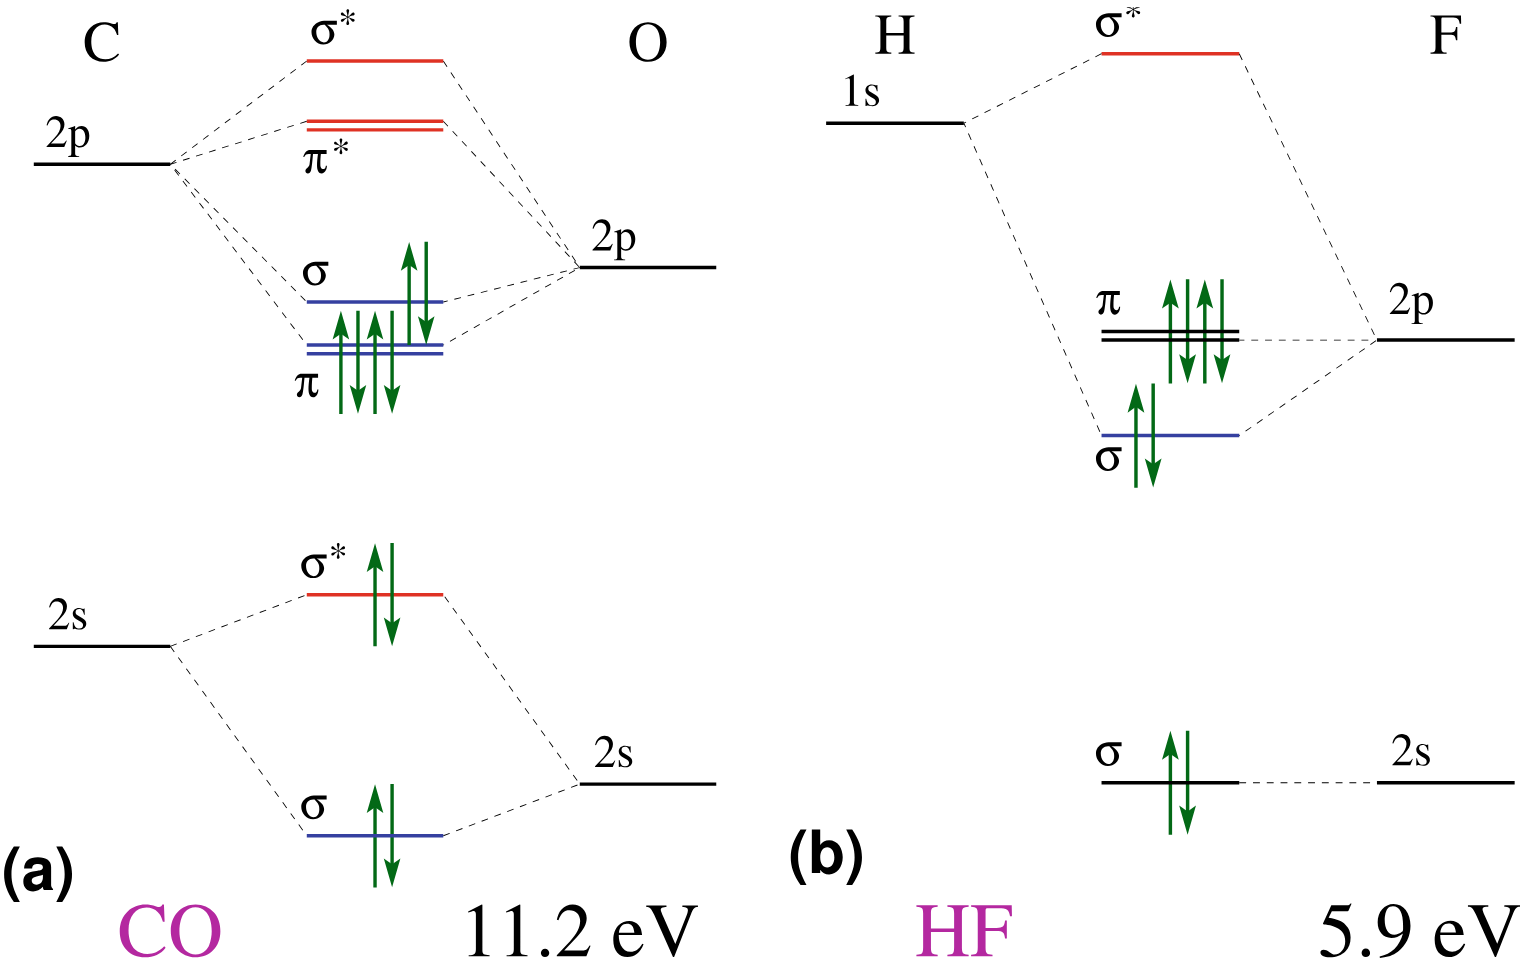
\includegraphics[width = 0.50 \textwidth]{eteronuclear.png}
	\caption{Bonding orbitals for eteronuclear diatomic molecules.}
	\label{etero}
\end{figure}

\subsection{Classificazione}

Nonostante la generale tendenza degli atomi ad attrarsi a grandi distanze e respingersi a corte distanze (Fig. \ref{ad-pot}), ci sono grosse differenze di distanze di equilibrio e profondità della buca di potenziale per i vari meccanismi di legame. \\
Se uno (o entrambi) dei due atomi è un gas nobile, allora il legame è di tipo dipolo-dipolo indotto (van der Waals), con una distanze d'equilibrio $ R_\text{m} \sim 250-400 \,\text{pm} $ grande ed energia di legame nell'ordine dei $ \text{meV} $. I gas nobili mantengono la forma di gas monoatomico fino a temperature relativamente basse, per poi formare dimeri in grado di condensarsi e solidificarsi. \\
Al contrario, alcuni atomi con shell non complete ($ \ch{N} $, $ \ch{O} $, $ \ch{F} $) tendono a formare molecole diatomiche con legami covalenti corti e molto forti (binding energy $ \sim \text{eV} $), molecole mantenute anche nelle fasi liquide e solide a basse temperature. Per la maggior parte degli altri atomi, l'energia extra guadagnata formando legami chimici multipli rende energeticamente conveniente formare legami metallici estesi (o anche solidi covalenti), piuttosto che molecole diatomiche.\\
Nel caso di molecole eteronucleari fortemente polari si può arrivare alla formazione di legami ionici, con un transferimento (totale o parziale) di carica da un'atomo all'altro: al pari dei legami covalenti e metallici, le distanze d'equilibrio sono $ R_\text{m} \sim 80-250 \,\text{pm} $ e le binding energies $ \sim 1-10\ev $.

\section{Spettri molecolari}

Si passa ora allo studio del moto dei due nuclei di una molecola diatomica, governato dall'Eq. \ref{eq:mol-nucl-eq}. Si noti che il potenziale adiabatico è indipendente dalla posizione del centro di massa della molecola (invarianza per traslazioni) e dall'orientazione nello spazio dell'asse molecolare (invarianza per rotazioni): di conseguenza, si può separare il moto in moto del centro di massa, che risulta in uno spettro continuo (il moto termico randomico del centro di massa genera l'allargamento delle linee spettrali per effetto Doppler), e moto relativo, il quale gode di simmetria sferica rispetto a $ \ve{R}_{12} $. Per quanto riguarda ques'ultimo, tramite la separazione delle variabili si può separare l'equazione nucleare in tre equazioni, di cui due angolari standard ed una radiale con potenziale adiabatico. Le soluzioni delle equazioni angolari sono le armoniche sferiche $ Y_{\ell,m_\ell} $, dove $ \ell $ è il momento angolare molecolare ed $ m_\ell \in [-\ell,\ell] $ la sua proiezione lungo l'asse molecolare. Per quanto riguarda l'equazione radiale, invece, data dall'Eq. \ref{eq:1-e-rad-eq} con $ V(r) \equiv V_\text{ad}(r) $ (ed $ r \equiv R_{12} $), si può considerare che il potenziale adiabatico presenta un minimo in in un punto d'equilibrio finiro $ R_{12} = R_\text{m} > 0 $, dunque si può considerare che la molecola studiata si trovi in un intorno di $ R_\text{m} $, così da poter ignorare variazioni del termine centrifugo $ \frac{\hbar^2 \ell (\ell + 1)}{2\mu R_{12}^2} $ ($ R_{12}^{-2} $ varia poco in un intorno di $ R_\text{m} > 0 $) ed approssimare il moto radiale come indipendente da $ \ell $; espandendo il potenziale attorno ad $ R_\text{m} $:
\begin{equation*}
	V_\text{ad}(R_{12}) = V_\text{ad}(R_\text{m}) + \frac{1}{2} \frac{d^2 V_\text{ad}(R)}{dR^2}\bigg\vert_{R = R_\text{m}} (R_{12} - R_\text{m})^2 + \dots \equiv V_\text{ad}(R_\text{m}) + \frac{1}{2} \kappa (R_{12} - R_\text{m})^2 + \dots
\end{equation*}
Si può dunque approssimare il potenziale con un potenziale armonico ed il sistema con un oscillatore armonico; definendo il numero quantico $ v \in \N_0 $ come il numero di nodi della funzione d'onda radiale, si trova lo spettro radiale vibrazionale:
\begin{equation}
	E_\text{vib}(v) = \hbar \omega \left( v + \frac{1}{2} \right)
\end{equation}
con $ \omega \equiv \sqrt{\kappa / \mu} $. Grandezze tipiche sono $ \hbar \omega \sim 20-400 \,\text{meV} $. Il termine centrifugo, invece, determina uno spettro rotazionale:
\begin{equation}
	E_\text{rot}(\ell) = \frac{\hbar^2 \ell (\ell + 1)}{2\mu R_\text{m}^2} \equiv \frac{\ve{L}^2}{2I}
\end{equation}
Questa è la cosiddetta approssimazione del rotatore rigido, in cui si definisce il momento d'inerzia $ I $: ciò è possibile poiché si è assunto che $ R_{12} \approx R_\text{m} $ privo di variazioni in un intorno di $ R_\text{m} $. Grandezze tipiche sono nell'ordine dei $ \text{meV} $: l'energia rotazionale più alta è quella del $ \ch{H_2} $, pari a $ 7 \,\text{meV} $.

\subsection{Spettro rotazionale e roto-vibrazionale}

Se si considerano transizioni adiabatiche, ovverosia transizioni in cui gli elettroni rimangono nel loro ground state, le molecole soddisfano le solite selection rules di dipolo elettrico: $ \Delta \ell = \pm 1 $.
Nel caso delle molecole diatomiche, l'operatore di dipolo elettrico è determinato dalla separazione tra i due nuclei e dalla loro differenza di carica: nel caso di molecole omonucleari tale differenza è nulla, dunque per esse non si osservano transizioni di dipolo elettrico\footnote{Questo è il motivo per cui l'aria (composta principalmente da $ \ch{N_2} $ e $ \ch{O_2} $) è altamente trasparente ai raggi IR; la trasparenza nel visibile e nel vicino UV è invece associata al grosso gap (vari $ \text{eV} $) che separa il ground state elettronico ed il primo stato eccitato elettronico.}. Inoltre, l'operatore di dipolo elettrico dipende dalla distanza $ R_{12} $: in un intorno di $ R_\text{m} $, si può espandere come:
\begin{equation*}
	\ve{d}(R_{12}) = \ve{d}(R_\text{m}) + \frac{\dd \ve{d}(R)}{\dd R}\bigg\vert_{R = R_\text{m}} (R_{12} - R_\text{m}) + \dots
\end{equation*}
In questo modo, come prima si erano eliminate le anarmonicità meccaniche, ora si sono eliminate le anarmonicità elettriche. Il termine costante $ \ve{d}(R_\text{m}) $ dà luogo allo spettro rotazionale puro (poiché $ \braket{\text{f} | \ve{d}(R_\text{m}) | \text{f}} \neq 0 $ solo se $ v_\text{f} = v_\text{i} $), mentre il termine proporzionale a $ R_{12} - R_\text{m} $ determina lo spettro roto-vibrazionale\footnote{Più precisamente, il termine $ \sim (R_{12} - R_\text{m})^n $ ha elemento di matrice non-nullo solo se $ v_\text{f} - v_\text{i} = \pm n $.}. \\
Gli spettri rotazionali e vibrazionali delle molecole si osservano principalmente come spettri d'assorbimento, dato che il basso rate di emissione spontanea (decay rate $ \sim \mathcal{E}_\text{if}^3 $) determina una preponderanza di fenomeni di decadimento radiation-less (es.: collisioni tra molecole).

\subsubsection{Spettro rotazionale}

Gli spettri puramente rotazionali si osservano nella regione del lontano IR e sono associati a transizioni con $ \Delta v = 0 $ e $ \Delta \ell = \pm 1 $. La differenza energetica tra $ \ket{\ell_\text{i}} \equiv \ket{\ell} $ e $ \ket{\ell_\text{f}} \equiv \ket{\ell + 1} $ è:
\begin{equation}
	\Delta E_\text{rot}(\ell) = \frac{\hbar^2}{I} (\ell + 1)
\end{equation}
Di conseguenza, lo spettro rotazionale di un campione di molecole in vari stati rotazionali iniziali sarà composto da una serie di righe d'assorbimento equispaziate, con una separazione energetica $ \hbar^2 / I $ che è il doppio della tipica scala energetica rotazionale $ \hbar^2 / 2I $. Una misura di tale separazione permette di stimare $ I $ e, di conseguenza, la distanza interatomica d'equilibrio $ R_\text{m} $. \\
L'equispaziatura dei salti energetici rotazionali permette di definire una \textit{temperatura rotazionale}, determinata da tale scala energetica:
\begin{equation}
	\theta_\text{rot} \defeq \frac{\hbar^2}{I k_\text{B}}
\end{equation}
dove $ k_\text{B} = 8.617 \cdot 10^{-5} \ev/\text{K} $ è la costante di Boltzmann. La scala di temperatura tipica è $ \sim 12 \,\text{K} $ (per energie $ \sim 1 \,\text{meV} $). Questa temperatura va confrontata con quella a cui si svolge l'esperimento: se $ T \ll \theta_\text{rot} $ il sistema si troverà sostanzialmente nel suo ground state, mentre se $ T \gg \theta_\text{rot} $ saranno popolati con buona probabilità molti livelli eccitati.

\begin{figure}
	\centering
	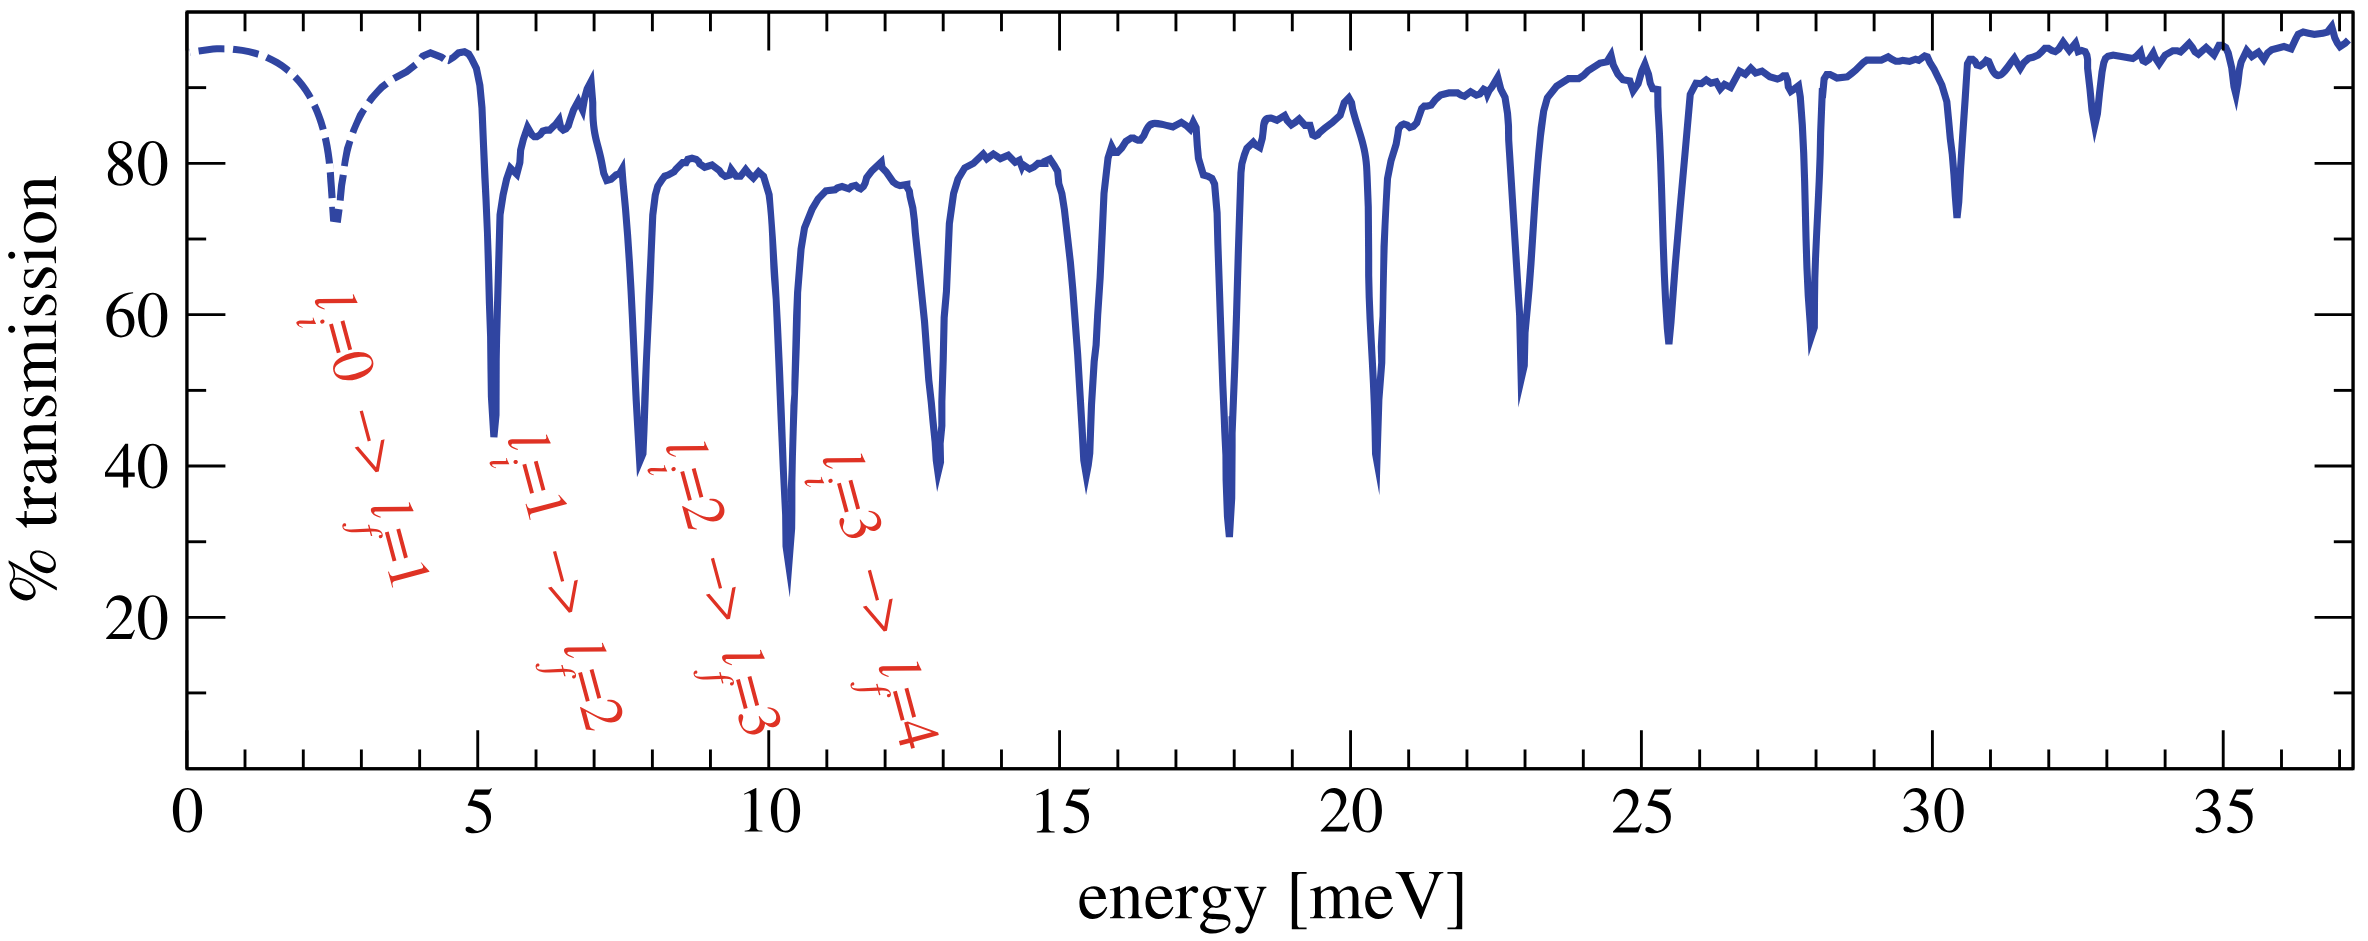
\includegraphics[width = 0.80 \textwidth]{rot-spectr.png}
	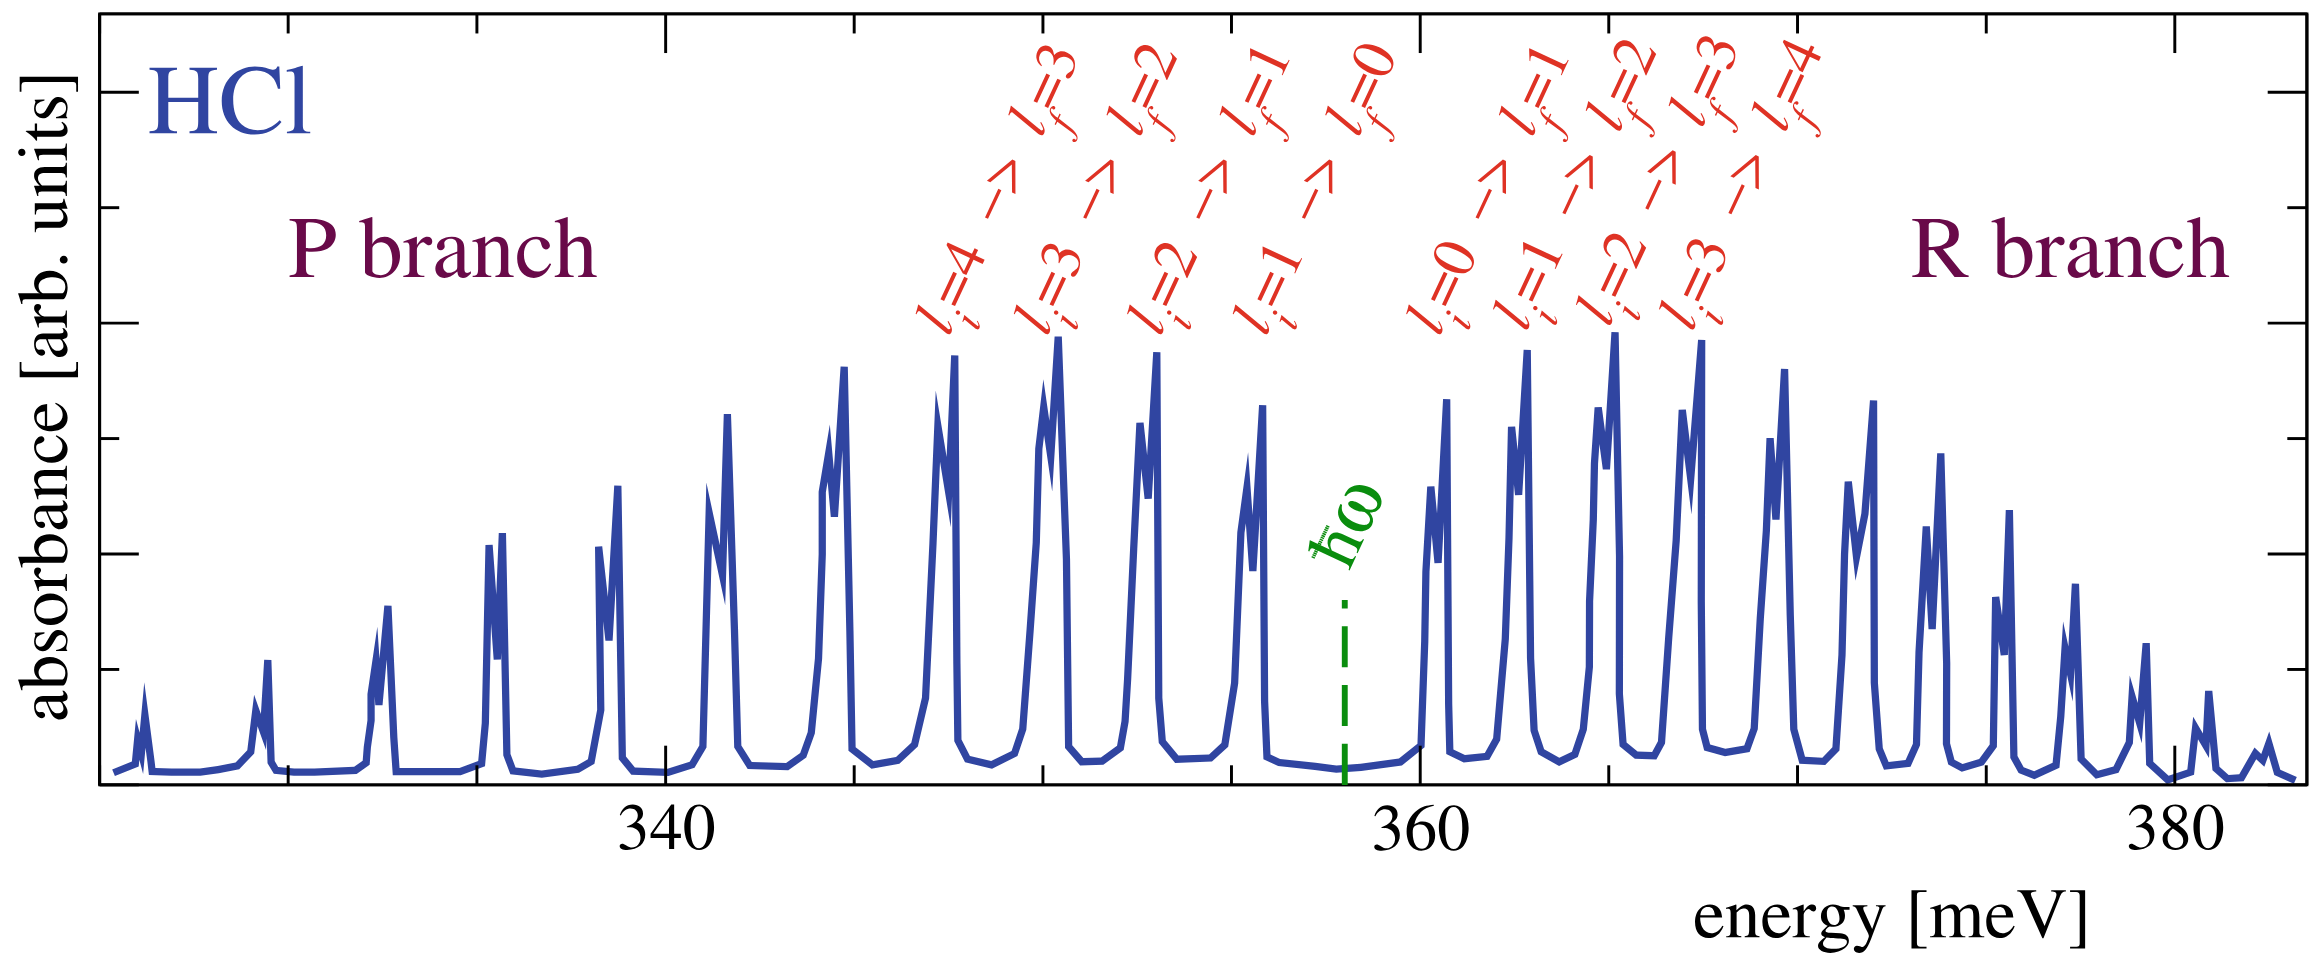
\includegraphics[width = 0.80 \textwidth]{rot-vib-spectr.png}
	\caption{Observed purely-rotational (above) and roto-vibrational (below) absorption spectrum of gas-phase $ \ch{HCl} $.}
	\label{rot-vib-sp}
\end{figure}
\begin{figure}
	\centering
	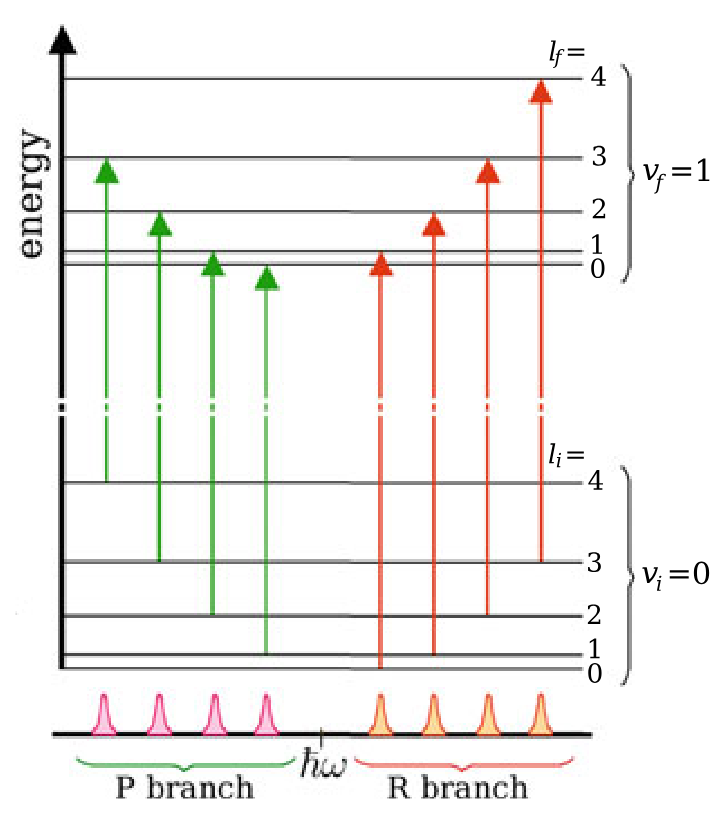
\includegraphics[width = 0.40 \textwidth]{rot-vib-spectr-det.png}
	\caption{Scheme of electric-dipole transitions between rotational levels $ \ket{v = 0} \rightarrow \ket{v = 1} $.}
	\label{rot-vib-det}
\end{figure}

\subsubsection{Spettro roto-vibrazionale}

Gli spettri roto-vibrazionali si osservano nella regione del vicino IR e sono associati a transizioni $ \Delta v > 0 $ e $ \Delta \ell = \pm 1 $: la maggior parte dell'intensità è data dalle transizioni $ \Delta v = 1 $, mentre le overtone transitions $ \Delta v > 1 $ sono più deboli. \\
Come si vede in Figg. \ref{rot-vib-sp}-\ref{rot-vib-det}, una volta fissata una transizione con $ \Delta v = 1 $, essa è $ \virgolette{decorata} $ da varie transizioni $ \Delta \ell = \pm 1 $, essendo il campione composto di molecole in vari stati rotazionali iniziali: le transizioni con $ \Delta \ell = -1 $ formalo la P-branch, mentre quelle con $ \Delta \ell = +1 $ la R-branch. Si noti l'assenza di una transizione piccata in $ \hbar \omega $, la quale sarebbe associata ad una transizione dipolo-proibita $ \Delta \ell = 0 $. \\
In presenza di uno spettrometro a bassa risoluzione, non si riescono a distinguere le singole righe rotazionali e si osserva un'unica riga vibrazionale. \\
Analogamente allo spettro rotazionale, si può definire una \textit{temperatura vibrazionale}:
\begin{equation}
	\theta_\text{vib} \defeq \frac{\hbar \omega}{k_\text{B}}
\end{equation}
In questo caso le energie si attestano su $ \sim 0.5\ev $, dunque $ \theta_\text{vib} \sim 6000 \,\text{K} $.

\subsubsection{Molecole poliatomiche}

Nel caso di molecole poliatomiche, in generale il potenziale adiabatico dipenderà sia dalle distanze relative tra i vari nuclei che dagli angoli tra tali distanze, rendendo la trattazione del problema molto più complessa. In particolare, ci saranno vari modi normali d'oscillazione attorno al minimo multidimensionale di $ V_\text{ad} $, ciascuno modellabile da un oscillatore armonico indipendente.

\subsection{Eccitazioni elettroniche}

Fotoni nel range del visibile e UV possono provocare eccitazioni dello stato elettronico delle molecole: queste eccitazioni possono essere modellate dalla promozione di un elettrone da un orbitale molecolare occupato ad uno vuoto. Una transizione $ \psi_e^{(a)} \rightarrow \psi_e^{(b)} $ provoca un cambiamento di superficie potenziale adiabatica: data la time-scale estremamente piccola, i nuclei non hanno tempo di muoversi, dunque (come in Fig. \ref{elec-ex}) tale cambiamento è $ \virgolette{verticale} $ in $ R_{12} $. Dato che in generale $ R_\text{m}^{(a)} \neq R_\text{m}^{(b)} $, solitamente le transizioni elettroniche sono accompagnate da transizioni vibrazionali dovute alla variazione della geometria d'equilibrio.

\begin{figure}
	\centering
	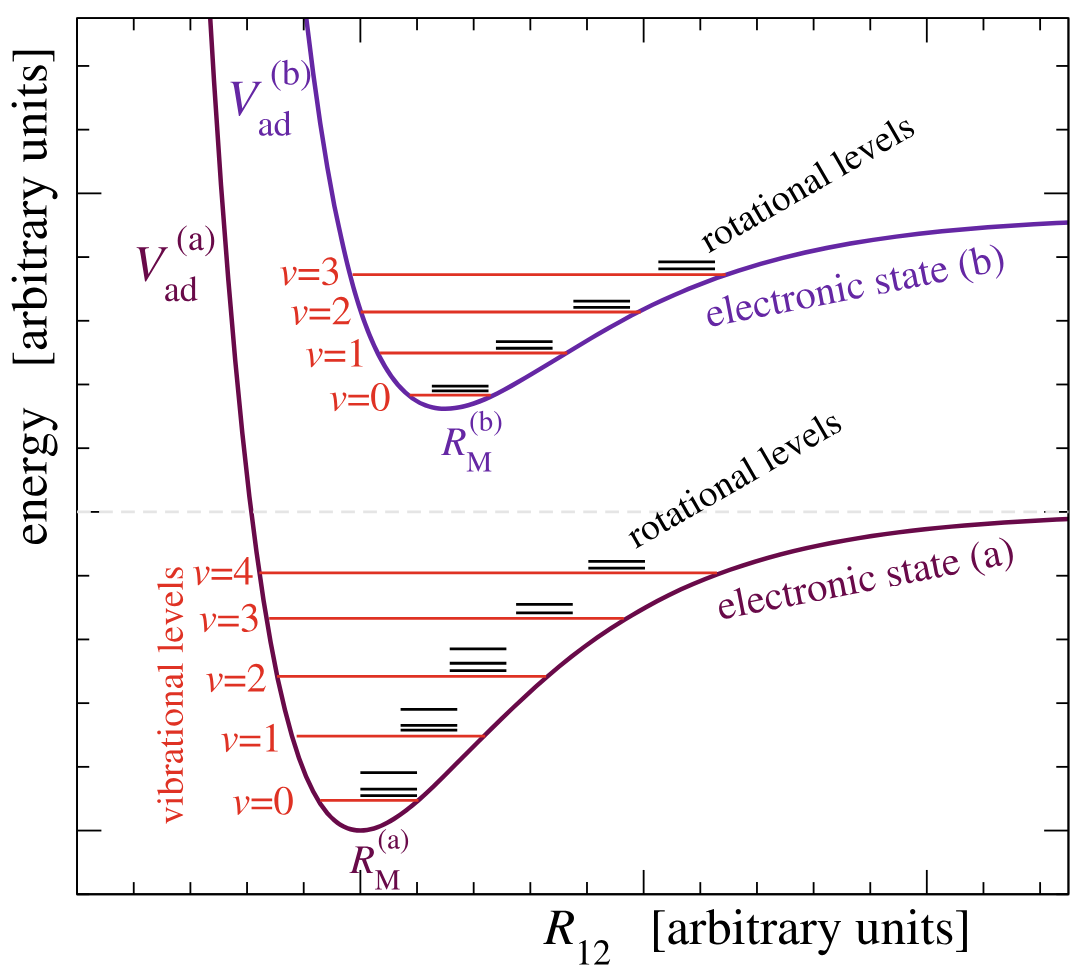
\includegraphics[width = 0.50 \textwidth]{electr-exc.png}
	\caption{Adiabatic potential surfaces for $ \psi_e^{(a)} \rightarrow \psi_e^{(b)} $.}
	\label{elec-ex}
\end{figure}
\begin{figure}
	\centering
	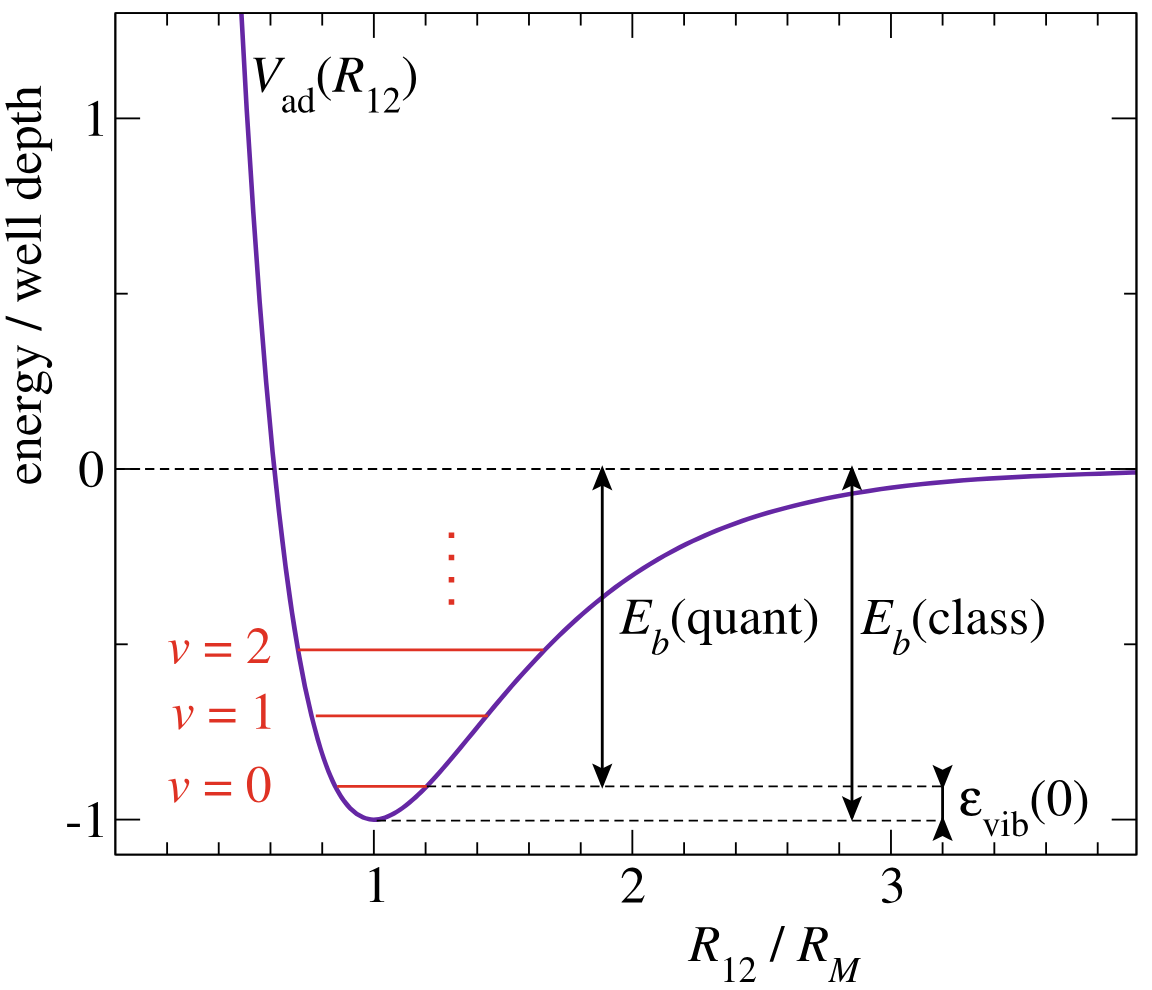
\includegraphics[width = 0.50 \textwidth]{zero-point-eff.png}
	\caption{Quantum zero-point vibrational energy.}
	\label{zero-p}
\end{figure}

\subsubsection{Effetti di punto-zero}

Come si vede in Fig. \ref{zero-p}, la binding energy $ E_b $ di una molecola diatomica è leggermente inferiore alla profondità $ V_\text{ad}(\infty) - V_\text{ad}(R_\text{m}) $ della buca di potenziale adiabatico. I due valori coinciderebbero se le masse dei nuclei fossero infinite (o se essi fossero oggetti classici), ma per il principio d'indeterminazione è presente un'energia vibrazionale di punto-zero $ E_\text{vib}(0) = \frac{\hbar \omega}{2} $, la quale spiega la piccola differenza tra i due valori. \\
Sperimentalmente, si possono indagare questi effetti di punto-zero andando a variare la massa degli isotopi coinvolti, dato che $ \omega \propto \mu^{-1/2} $ mentre $ V_\text{ad}(R_{12}) $ non dipende da esso. Uno degli effetti di punto-zero più grandi si ha nel $ \ch{^4He_2} $: la buca di potenziale adiabatico è profonda circa $ 900 \,\mu\text{eV} $, ma il sistema è estremamente debolmente legato con $ E_b \simeq 0.1 \,\mu\text{eV} $, dunque $ E_\text{vib}(0) $ bilancia quasi completamente l'attrazione adiabatica. A confermare la dipendenza da $ \mu $, per il più leggero $ \ch{^3He_2} $ non si osservano stati legati (l'energia di punto-zero è più grande della buca di potenziale adiabatico).











